%%%%%%%%%%%%%%%%%%%%%%%%%%%%%%%%%%%%%%%%%%%%%%%%%%%%%%%%%%%%%%%%%%%%%%
% Problem statement
\begin{statement}[
  problempoints=100,
  timelimit=1 sekunda,
  memorylimit=1024 MiB,
]{Sirologija}

Vi ste mrav, i to ne običan mrav već mrav opsjednut sirologijom!

Otkrili ste novu krišku sira u kuhinji, te želite poslati što više svojih podanika kako bi istražili sir. Sir možemo zamisliti kao tablicu s $N$ redaka i $M$ stupaca gdje su redci označeni brojevima od $1$ do $N$ odozgo prema dolje i stupci označeni brojevima od $1$ do $M$ s lijeva prema desno. Neka polja sadrže rupe, dok su ostala sir. Polje u $r$-tom retku i $s$-tom stupcu označavat ćemo kao $(r, s)$. U gornjem lijevom polju i donjem desnom polju će se sigurno nalaziti sir.

Označimo broj podanika s $K$. Vaši podanici započet će svoju istragu u gornjem lijevom polju te ga završiti u donjem desnom polju. Mogu se kretati samo u smjerovima dolje i desno. Dodatno, njihovi putevi se ne smiju "sjeći" tj. možemo im dodijeliti oznake od $1$ do $K$ tako da ne postoji polje iz kojega je podanik s manjom oznakom izašao prema desno, a podanik s većom oznakom prema dolje.

Također, htjeli biste da su ti putevi ipak u nekom smislu "različiti", tj. da za svaka dva podanika postoji polje $(r, s)$ u kojem se nalazi rupa, tako da se jedan od njih u nekom trenutku nalazio u stupcu $s$ te retku s oznakom manjom od $r$, a drugi u nekom trenutku (ne nužno istom) nalazio u stupcu $s$ te retku s oznakom većom od $r$. Neformalno, svaka dva podanika su neku rupu obišli s različitih strana.

Ispišite najveći $K$ takav da postoji odabir putanja podanika koje zadovoljavaju tražene uvjete.

Neki primjeri puteva koji ne zadovoljavaju uvjete:

\begin{figure}[!h]
    \centering
    \begin{subfigure}{0.49\linewidth}
      \centering
      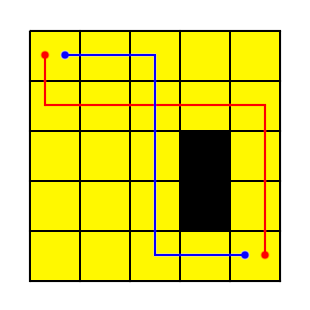
\includegraphics[width=\linewidth]{pic/sijeku_se.png}
      \caption{Loš odabir puteva - sijeku se}

    \end{subfigure}
    \begin{subfigure}{0.49\linewidth}
      \centering
      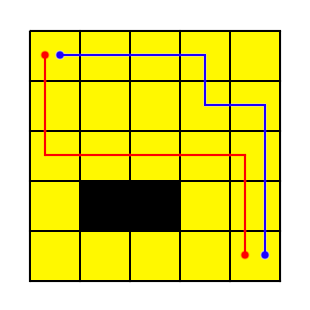
\includegraphics[width=\linewidth]{pic/ista_strana.png}
      \caption{Loš odabir puteva - obilaze rupu s iste strane}

    \end{subfigure}

  \end{figure}

%%%%%%%%%%%%%%%%%%%%%%%%%%%%%%%%%%%%%%%%%%%%%%%%%%%%%%%%%%%%%%%%%%%%%%
% Input
\subsection*{Ulazni podaci}

U prvom su retku prirodni brojevi $N$, $M$.

U sljedećih $N$ redaka nalaze se opisi redaka tablice. U $i$-tom se retku nalazi $M$ znakova gdje $\texttt{.}$ označava sir dok $\texttt{\#}$ označava polje koje sadrži rupu. 

%%%%%%%%%%%%%%%%%%%%%%%%%%%%%%%%%%%%%%%%%%%%%%%%%%%%%%%%%%%%%%%%%%%%%%
% Output
\subsection*{Izlazni podaci}

U jedini redak ispišite najveću moguću vrijednost broja $K$.

%%%%%%%%%%%%%%%%%%%%%%%%%%%%%%%%%%%%%%%%%%%%%%%%%%%%%%%%%%%%%%%%%%%%%%
% Scoring
\subsection*{Bodovanje}

U svim podzadacima vrijedi $2 \leq N, M \leq 2000$.

{\renewcommand{\arraystretch}{1.4}
  \setlength{\tabcolsep}{6pt}
  \begin{tabular}{ccl}
   Podzadatak & Broj bodova & Ograničenja \\ \midrule
    1 & 15 & Sve rupe nalaze se u istom retku. \\
    2 & 18 & $N, M \leq 10$ \\
    3 & 16 & $N, M \leq 50$, ne postoji rupa u prvom ili zadnjem retku te prvom ili zadnjem stupcu.\\
    4 & 18 & $N, M \leq 50$ \\
    5 & 16 & $N, M \leq 2000$, ne postoji rupa u prvom ili zadnjem retku te prvom ili zadnjem stupcu.\\
    6 & 17 & Nema dodatnih ograničenja. \\
\end{tabular}}

%%%%%%%%%%%%%%%%%%%%%%%%%%%%%%%%%%%%%%%%%%%%%%%%%%%%%%%%%%%%%%%%%%%%%%
% Examples
\subsection*{Probni primjeri}
\begin{tabularx}{\textwidth}{X'X'X}
\sampleinputs{test/sirologija.dummy.in.1}{test/sirologija.dummy.out.1} &
\sampleinputs{test/sirologija.dummy.in.2}{test/sirologija.dummy.out.2} &
\sampleinputs{test/sirologija.dummy.in.3}{test/sirologija.dummy.out.3}
\end{tabularx}

\textbf{Pojašnjenje probnih primjera:}\\

\begin{figure}[!h]
    \centering
    \begin{subfigure}{0.49\linewidth}
      \centering
      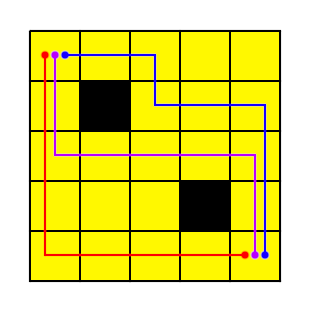
\includegraphics[width=\linewidth]{pic/sir.png}
      \caption{Primjer odabira puteva prvog primjera}

    \end{subfigure}
    \begin{subfigure}{0.49\linewidth}
      \centering
      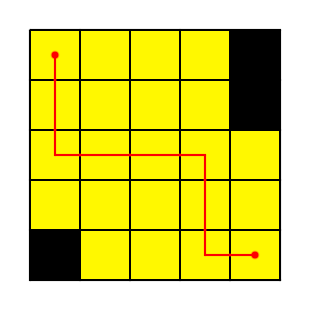
\includegraphics[width=\linewidth]{pic/sir2.png}
      \caption{Primjer odabira puteva drugog primjera}

    \end{subfigure}

  \end{figure}
  
%%%%%%%%%%%%%%%%%%%%%%%%%%%%%%%%%%%%%%%%%%%%%%%%%%%%%%%%%%%%%%%%%%%%%%
% We're done
\end{statement}

%%% Local Variables:
%%% mode: latex
%%% mode: flyspell
%%% ispell-local-dictionary: "croatian"
%%% TeX-master: "../hio.tex"
%%% End: